\section{What Caching is}



Making computers more efficient and responsive has been a goal of computer researchers and engineers since the inception of Computer Science. One struggle that persists today is the efficient and timely retrieval of data. Since there is no way to make data storage both fast and large, engineers created caching. The idea behind caching is to combine fast, small memory with large, slow memory to mimic memory that is both large and fast.

\begin{figure}[h]
    \centering
    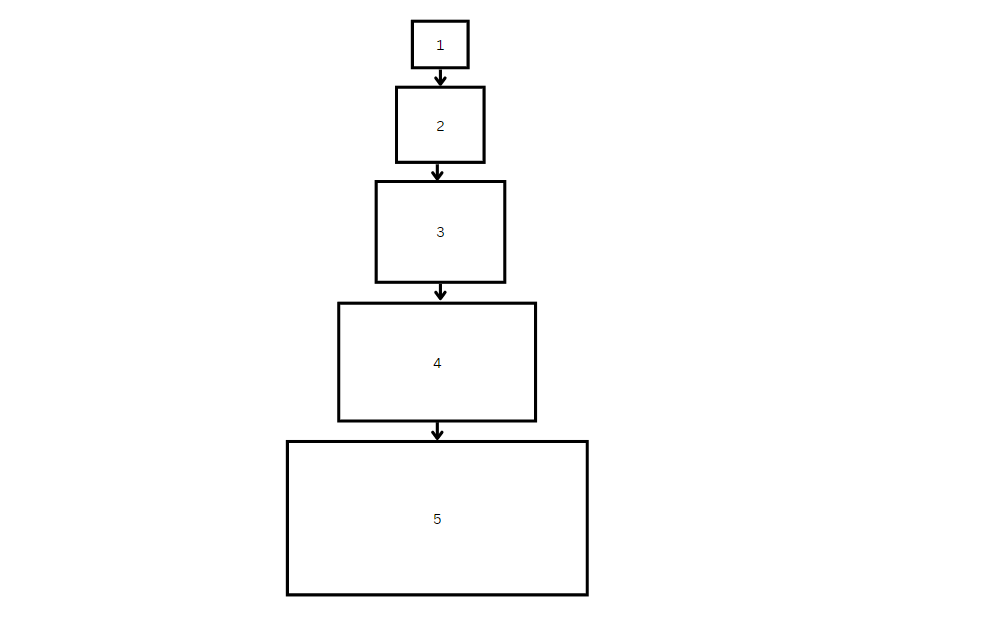
\includegraphics[scale=0.5, trim={0 .8cm 4cm 0cm},clip]{thesistemplate_2020-04-24/chapters/ch1 diagrams/cachesunFinal.png}
    \caption{A cache structure}
    \label{fig:my_label}
\end{figure}

In Figure 1.1, there are five levels of memory that grow physically larger as their level increases. This increase in size allows these higher levels to store more data but at the cost of the speed that the lower levels have. These levels are called caches. The problem with this approach is that caching only improves performance if the data being requested is in small fast memory. This is because, if the data is not in the small memory we must return to the state of a large slow memory.  


Since these small and fast caches can only store a subset of the data in the main memory, how do we ensure they store the requested data? They do this by taking advantage of a property called locality. Locality states that programs are likely to do two things: they are likely to reaccess data they have recently accessed and they are likely to access data near where they are accessing. This property means that the amount of data being accessed is usually small. 

Although we know that there is likely a small amount of relevant data, we still need to determine which data is relevant. In addition to this relevant data, caches quickly fill up with data that is not going to be relevant to future computations. When caches become full, decisions must be made regarding what data to keep versus what to discard from the cache. This process is called eviction.

These eviction decisions are done using cache algorithms, these algorithms decide what data is kept in the cache. There are many types of caches, which has led to a wide variety of cache algorithms with many different focuses.


When designing caching systems we would like to consider a variety of different design choices including which algorithm to use. However, implementing these choices in order to perform testing is very expensive. To avoid these costs, we turn to theoretical models. 


\section{Caching Models}

%TODO: 
To remove extraneous system details and focus on the problem of replacement, the abstract caching problem was created. It provides a way to analyze algorithms' performance without having to implement them.   

\begin{figure}[h]
    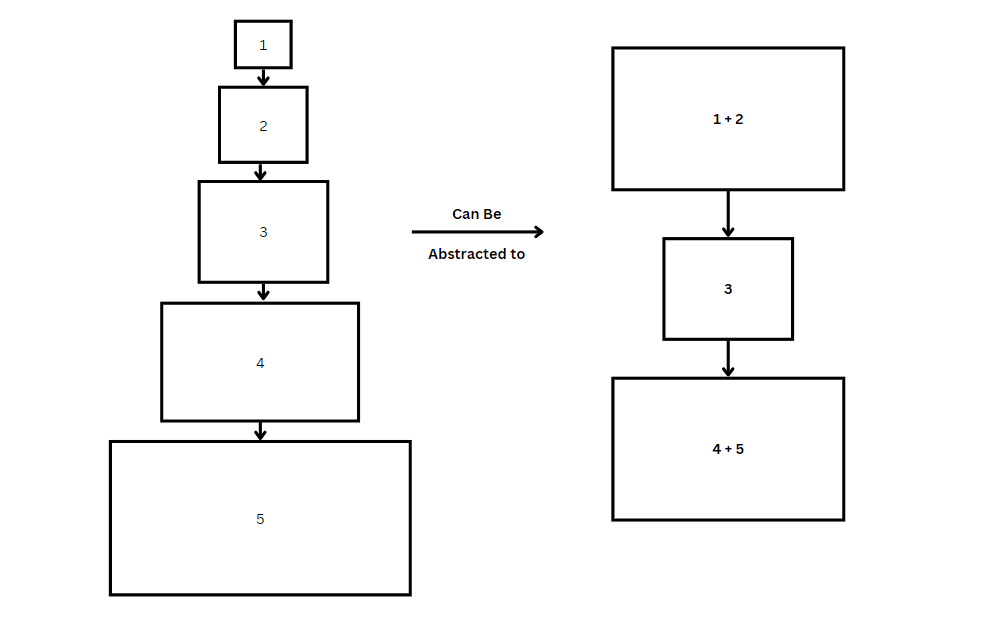
\includegraphics[scale=0.5,  trim={-2cm 0 4cm 0cm},clip]{thesistemplate_2020-04-24/chapters/ch1 diagrams/cachesabFinal.png}
    \caption{How we can view an abstract cache}
    \label{fig:my_label}
\end{figure}



Figure 1.1 shows a system with five levels of caches. An inefficient way to analyze this system would be to look at all five levels and their associated performances. Thinking of caches in the abstract frees us from having to look at all five levels of the cache. Instead, we choose one level of the cache and look at how it performs on a given trace of requests.


In Figure 1.2, we look at level 3 in the abstract model. Since we are focusing just on level 3, we only care about the requests that level 3 handles. This means we can abstract levels 1 and 2 into a single level, as they either already contained the requested data, or it wasn't present. If they contained the data, level 3 never sees the request regardless of which level contained it. Whereas if they didn't level 3 gets this request. We can use this same logic to abstract levels 4 and 5. Because we only care about level 3 and its performance, if level 3 didn't contain the data requested it doesn't matter if it is contained in level 4 or 5.

The abstract caching problem focuses on a cache of size $k$ given a trace $\sigma = \{i_{0}...i_{n} \}$, where each $i$ is requested one at a time in the order of the trace. Every item $i$ has an associated size $S(i)$ and cost $C(i)$. When an item is requested in this problem, the system can't proceed until the item is in the cache. While loading items, the total size of items in the cache can never exceed $k$
When items are requested, if the item is not in the cache, it must pay cost $C(i)$. For an item to fit in a cache, it must first evict items until it has $S(i)$ room.


 
\subsection{The Paging Model}
In the paging model, $\forall i \in \sigma  \text{ }cost(i) =  size(i)=1$. This means that on any given trace, all items' costs and sizes are equal. This model was introduced by \cite{sleator1985amortized} and was created to study cache storage. It allows researchers to look at processor caches wherein there is no size variation because the data is stored in the same size blocks. The cost of retrieving elements from memory is not considered as important as missing a request. 

\subsection{The Cost Model}
In the cost model, $\forall i \in \sigma \text{ } cost(i) =n \text{, } size(i)=1$. This means that any given trace, items will all have the same size, but can vary in cost. This was created by \cite{young1994k} to study the online k server problem in a new model. This model is useful for processor caches, where the size of items is always the same. Unlike the paging model, it can take into account the actual cost it takes to search for items in shared memory.


\subsection{The Fault Model}
In the fault model, $\forall i \in \sigma \text{ } cost(i) = 1\text{, } size(i)=(0\text{ to }k)$. This means that items will have a set cost, but can vary in size. This model was introduced by \cite{irani1997page} and was made to focus on the study of algorithms in web systems. This allows researchers to look at web caches, as the cost of a miss is so large on any item that they can all be considered equal.

\subsection{The Bit Model}
In the bit model, when given $\sigma$, $\forall i \text{ }cost(i)=size(i)$. This model was first introduced by \cite{irani1997page}. This means that items will have a cost that is equal to size. Irani created the model to study the effects of caching algorithms on web caches, but unlike the fault model, the cost difference can be taken into account. This allows bandwidth to be taken into consideration as larger files cost more to transfer.


\subsection{General Model}
In the general model of caching, when given $\sigma$, $\forall i, \textbf{ }  Cost(i) \text{, } Size(i)$. The sizes and costs are not constant between these different items, meaning that on any given trace, the items' sizes and costs can vary. This flexibility comes with an increase in complexity as in this model algorithms must balance the cost of items versus their size.